


\section{Introduction}

\begin{frame}
    \frametitle{Simulation}

    \begin{itemize}

        \item In simulation, pseudorandom numbers serve as the foundation for
        generating samples from probability distribution;

        \item Assume a \textbf{good random number generator} has been tested and that it 
        produces sequences of $U_I\sim~U(O,1)$ (uniform distribution);

        \item The goal is to produce samples $X_i$ from a distribution $F(x)$,
        giver a source of random numbers, $U_I\sim~U(0,1)$.

    \end{itemize}

\end{frame}


\begin{frame}
    \frametitle{Simulation}
    \begin{figure}
        \centering
        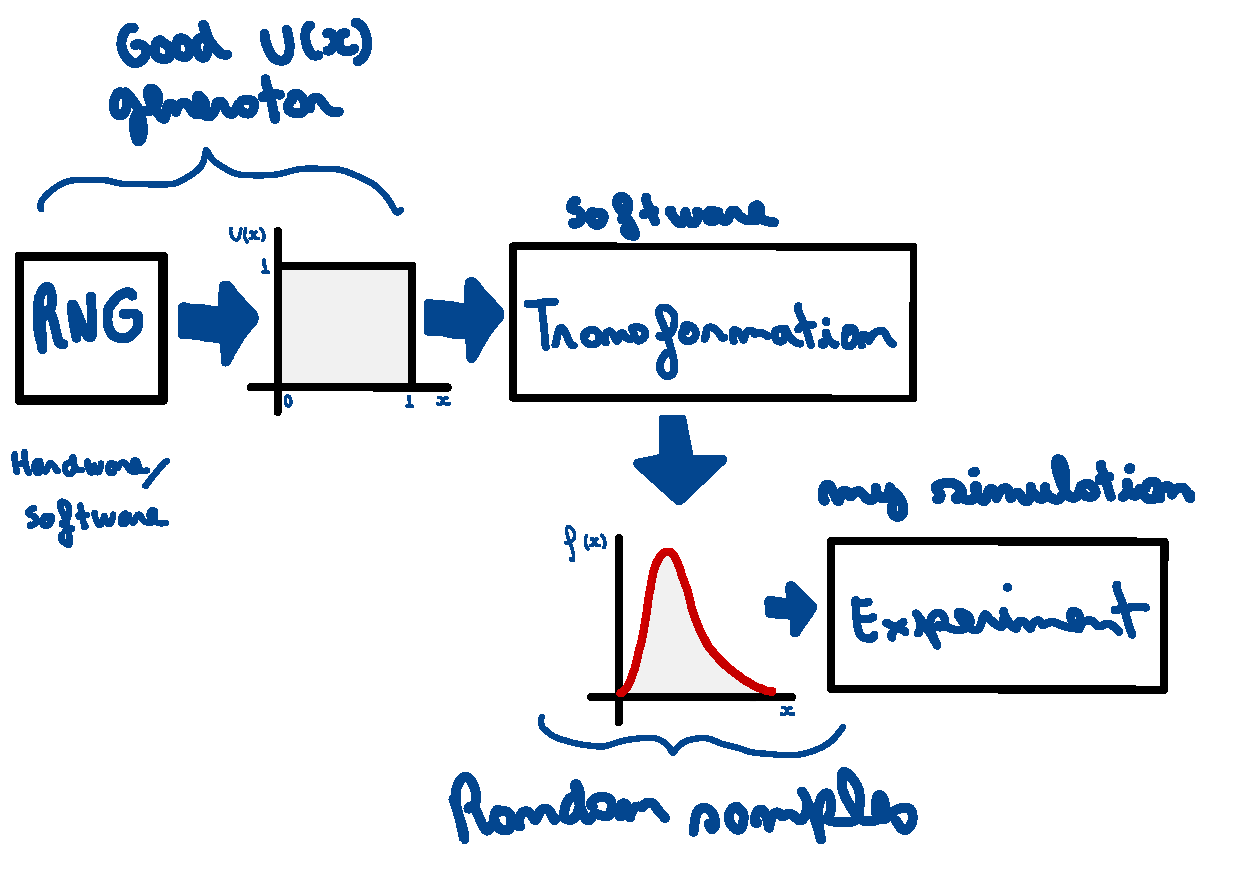
\includegraphics[width=0.95\textwidth]{sections/introduction/figures/simulation_framework.pdf}
    \end{figure}
\end{frame}


